\documentclass[]{MSword}
% Class options:
%-------------------------------
% nobib         - skip bibliography code/ don't include bib
% math          - include math packages and useful math commands
% hidelinks     - hide hyperref colored link boxes
% wordlinks     - link color scheme similar to word


% Preamble code:
%%%%%%%%%%%%%%%%%%%%%%%%%%%%%%%%%%%%%%%%
\usepackage[english]{babel}
\usepackage{csquotes}
\usepackage{lipsum}
\addbibresource{bib/bibliography.bib}

% % Uncomment using "Ctrl + /" (/ on numpad):
% % Customizing headers and footers:
% \fancypagestyle{custom}{%
%     \fancyhf{}% clears the footer and header
%     % Header:
%     \fancyhead[L]{}
%     \fancyhead[C]{}
%     \fancyhead[R]{}
%     % Footer:
%     \fancyfoot[L]{}
%     \fancyfoot[C]{}
%     \fancyfoot[R]{}
%         % Tips:
%         % ----
%         % L: left, C: center, R: right
%         % O: odd pages, E: even pages
%         % ----
%         % Example: \fancyghead[LO,RE]{Text}
%         % will produce "Text" left in the header
%         % on odd pages and right in the header on even pages.
%     % Rules/ lines:
%     \renewcommand{\headrulewidth}{0.4pt}
%     \renewcommand{\footrulewidth}{2pt}
% }
% % Changing the pagestyle:
% \pagestyle{custom}

%%%%%%%%%%%%%%%%%%%%%%%%%%%%%%%%%%%%%%%%

% Preamble information:
%%%%%%%%%%%%%%%%%%%%%%%%%%%%%%%%%%%%%%%%

\title{Background Research}
\author{Jerome Washo, Ben Wakefield}
\date{February 2023}

%%%%%%%%%%%%%%%%%%%%%%%%%%%%%%%%%%%%%%%%

% The document:
%%%%%%%%%%%%%%%%%%%%%%%%%%%%%%%%%%%%%%%%
\begin{document}

\maketitle
\begin{center}
    Words: \quickwordcount{main}\\ % Word count 
\end{center}

\section{Integrated Guitar Systems}
\par{There is a plethora of commercial products that have provided inspiration for the AxeTron. The primary product that has consistently been investigated by a multitude of companies is the MIDI guitar. A guitar that can be connected to a computer to control VSTs or to control MIDI supported pedals.}

\subsection*{Expressiv MIDI Pro 2}

\begin{center}
  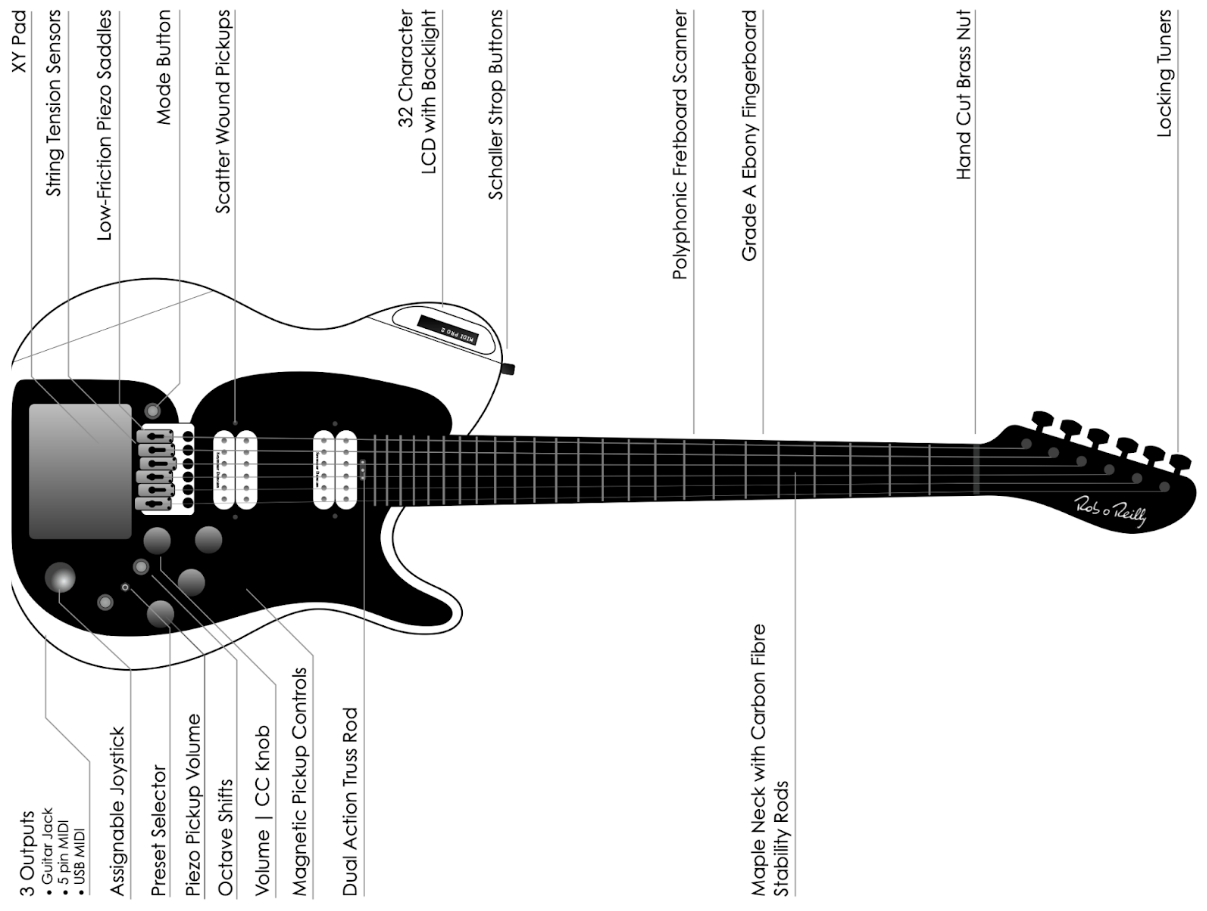
\includegraphics[width=0.5\textwidth]{img/expressiv.png}
\end{center}

\par{A highly-advanced MIDI guitar controller is the Expressiv MIDI Pro 2\cite{expressivmidi}, an elegant design from Rob O’Reilly guitars. It's also a dependable instrument, capable of producing audio. What separates this guitar from a traditional electric guitar is the variety of control surfaces that have been incorporated into the body of the instrument.}

\par{The physical controls on the guitar are 3 switches that can be progranned to a preset and also an octave or semitone transposition. Additionally, there is a double axis joystick that can be used as a pitch bend or can be programed to alter other effects. An XY pad that can be used for note triggering, velocity, Pitch bend, and can be used to control other parameters on pedals or in a DAW as well.}

\par{The XY pad is a feature that will be implemented on the AxeTron.  It’s a feature you would typical see on a synthesizer, but offers a variety of creative expression on a guitar. There are six pressure sensitive pads that can be customized to control any of your effects that you are using in your signal chain or in your DAW. These pressure sensitive pads are also compatible with aftertouch which is midi data that is produced from pressure being applied to the button. Aftertouch is an extremely expressive feature that would be exciting to add to the AxeTron.}

\par{The brains of the Expressiv MIDI Pro 2 are nothing crazy, but to see the performance from this guitar with such a small processor provides hope that our Daisy Seed will be overkill for our project. The processor is running at 16MHz and has an onboard memory capacity of 4KB. This lets the user set up to 30 presets on the guitar that can be seen through the 32 character LCD screen that it near the strap button on the guitar.}

\par{For a comparison, the Daisy Seed\cite{daisyseed} that we will be using has ARM Cortex-M7 which is running at 480 MHz and 64MB of SDRAM that allows for up to 10 minutes of audio buffers. Comparatively, the Daisy Seed should provide more than enough power for the AxeTron.}

\subsection*{Roland GS-500}

\begin{center}
  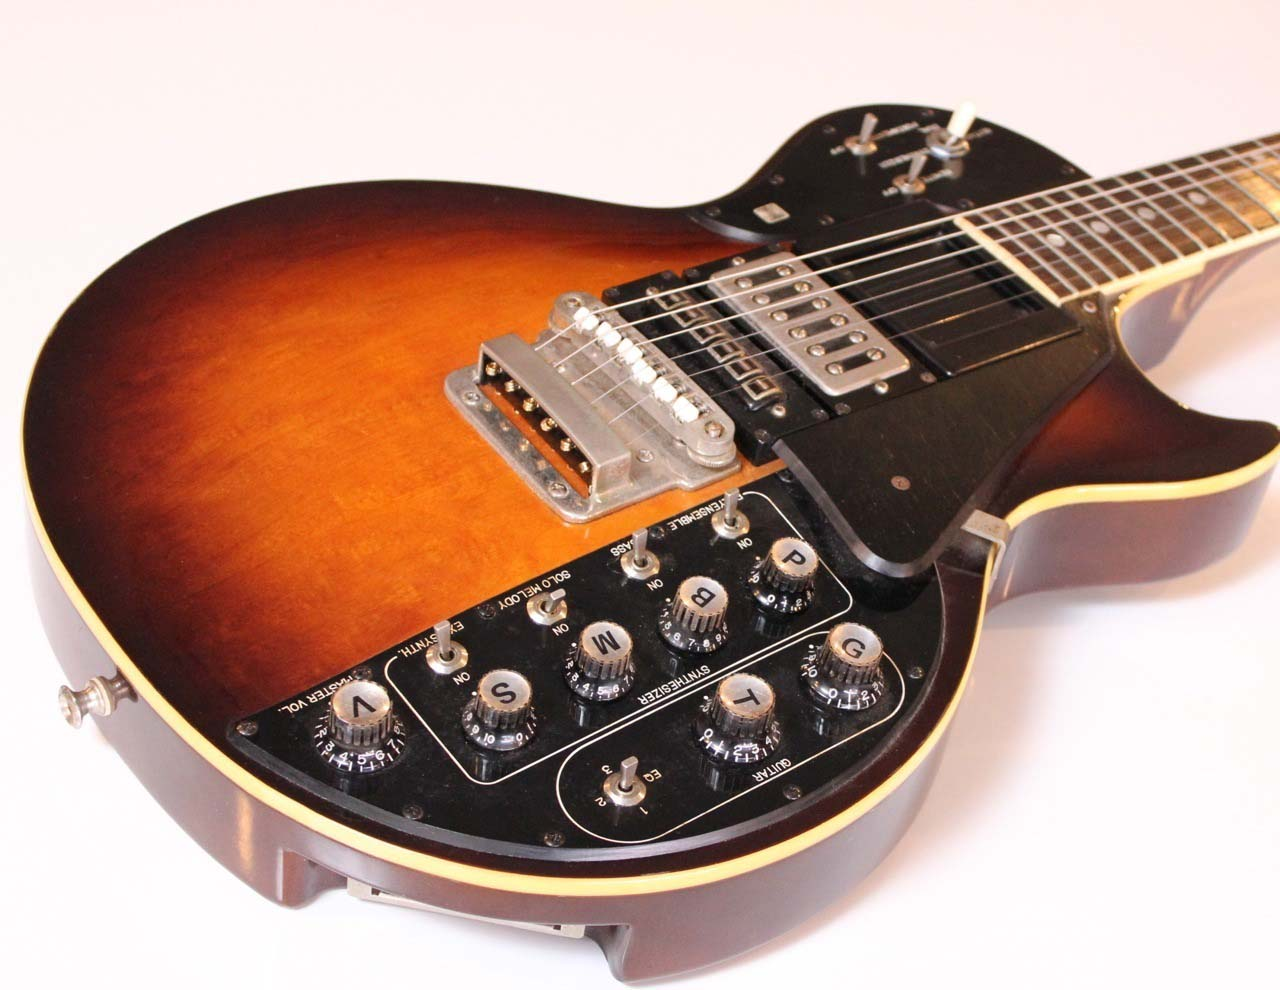
\includegraphics[width=0.5\textwidth]{img/rolandgs500.jpg}
\end{center}

\par{The Roland GS-500\cite{rolandgs500} was an early sign of what was possible in terms of guitar modification. This was  dedicated controller for the GS-500 synthesizer. The knob were all dedicated controls that could be found on the actual synthesizer, but additionally it had a 3 way switch EQ that was helpful to achieve different tones. The GS-500 controller only had one pickup so the EQ switches helped deliver the variety of tones you would get out of a traditionally electric guitar. One of the most unique features of this guitar was its ‘Infinite Sustain.’ It used two powerful magnets of opposite polarity and placed them outside the strings which created a strong magnetic field across the strings. The frets on the guitar are grounded to the strings behave according to the magnetic field. The guitar has a hexa-phonic pickup that pickups up the vibration of the string, amplifies the signal, and then the string continues to vibrate at the same frequency, thus creating the ‘Infinite Sustain.’}

\subsection*{Godwin Guitorgan}

\begin{center}
  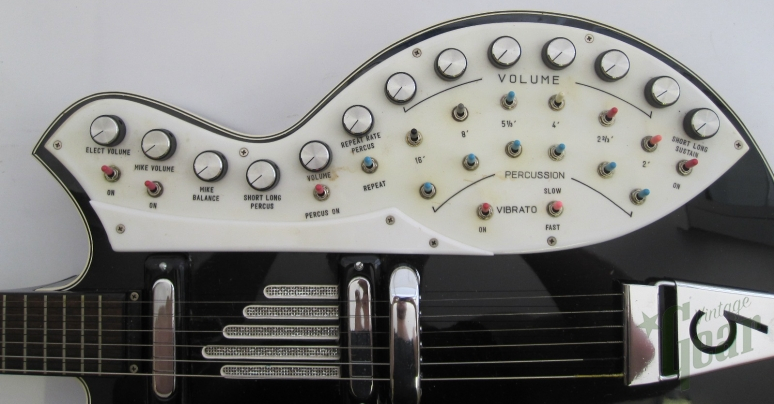
\includegraphics[width=0.5\textwidth]{img/guitorgan.png}
\end{center}

\par{The Godwin Guitorgan\cite{godwinguitorgan} is a fascinating instrument that is both rare and unique in its design. It was created in the 1970s by Robert Godwin, who was inspired by the original Gibson Guitorgan\cite{gibsonguitorgan} but sought to create an instrument that would offer an expanded range of organ sounds and greater control over those sounds.}

\par{The Godwin Guitorgan features six guitar strings and a bank of twelve organ keys, much like the Gibson Guitorgan. However, it also includes a variety of additional controls and features that make it a more versatile and expressive instrument. For example, it has an expanded set of organ voices that can be selected using a series of switches and buttons, allowing the player to create a wide range of tonal colors and textures. It also has a built-in Leslie speaker, which provides a distinctive rotary speaker effect that is commonly associated with the sound of classic Hammond organs.}

\par{Playing the Guitorgan requires a high degree of skill and coordination. The right hand is used to play the guitar strings, while the left hand is used to play the organ keys. The player's feet control various parameters, such as the volume and speed of the Leslie speaker, using a set of pedals.}

\par{Despite its technical complexity, the Guitorgan has been embraced by many musicians as a versatile and innovative instrument. The general concept of merging another instrument with an electric guitar is in line with our project. More specifically, the control layout serves as an inspiration for how the Daisy Seed effects unit might be controlled by the player.}

\section{Standalone Effects Units}

\begin{center}
  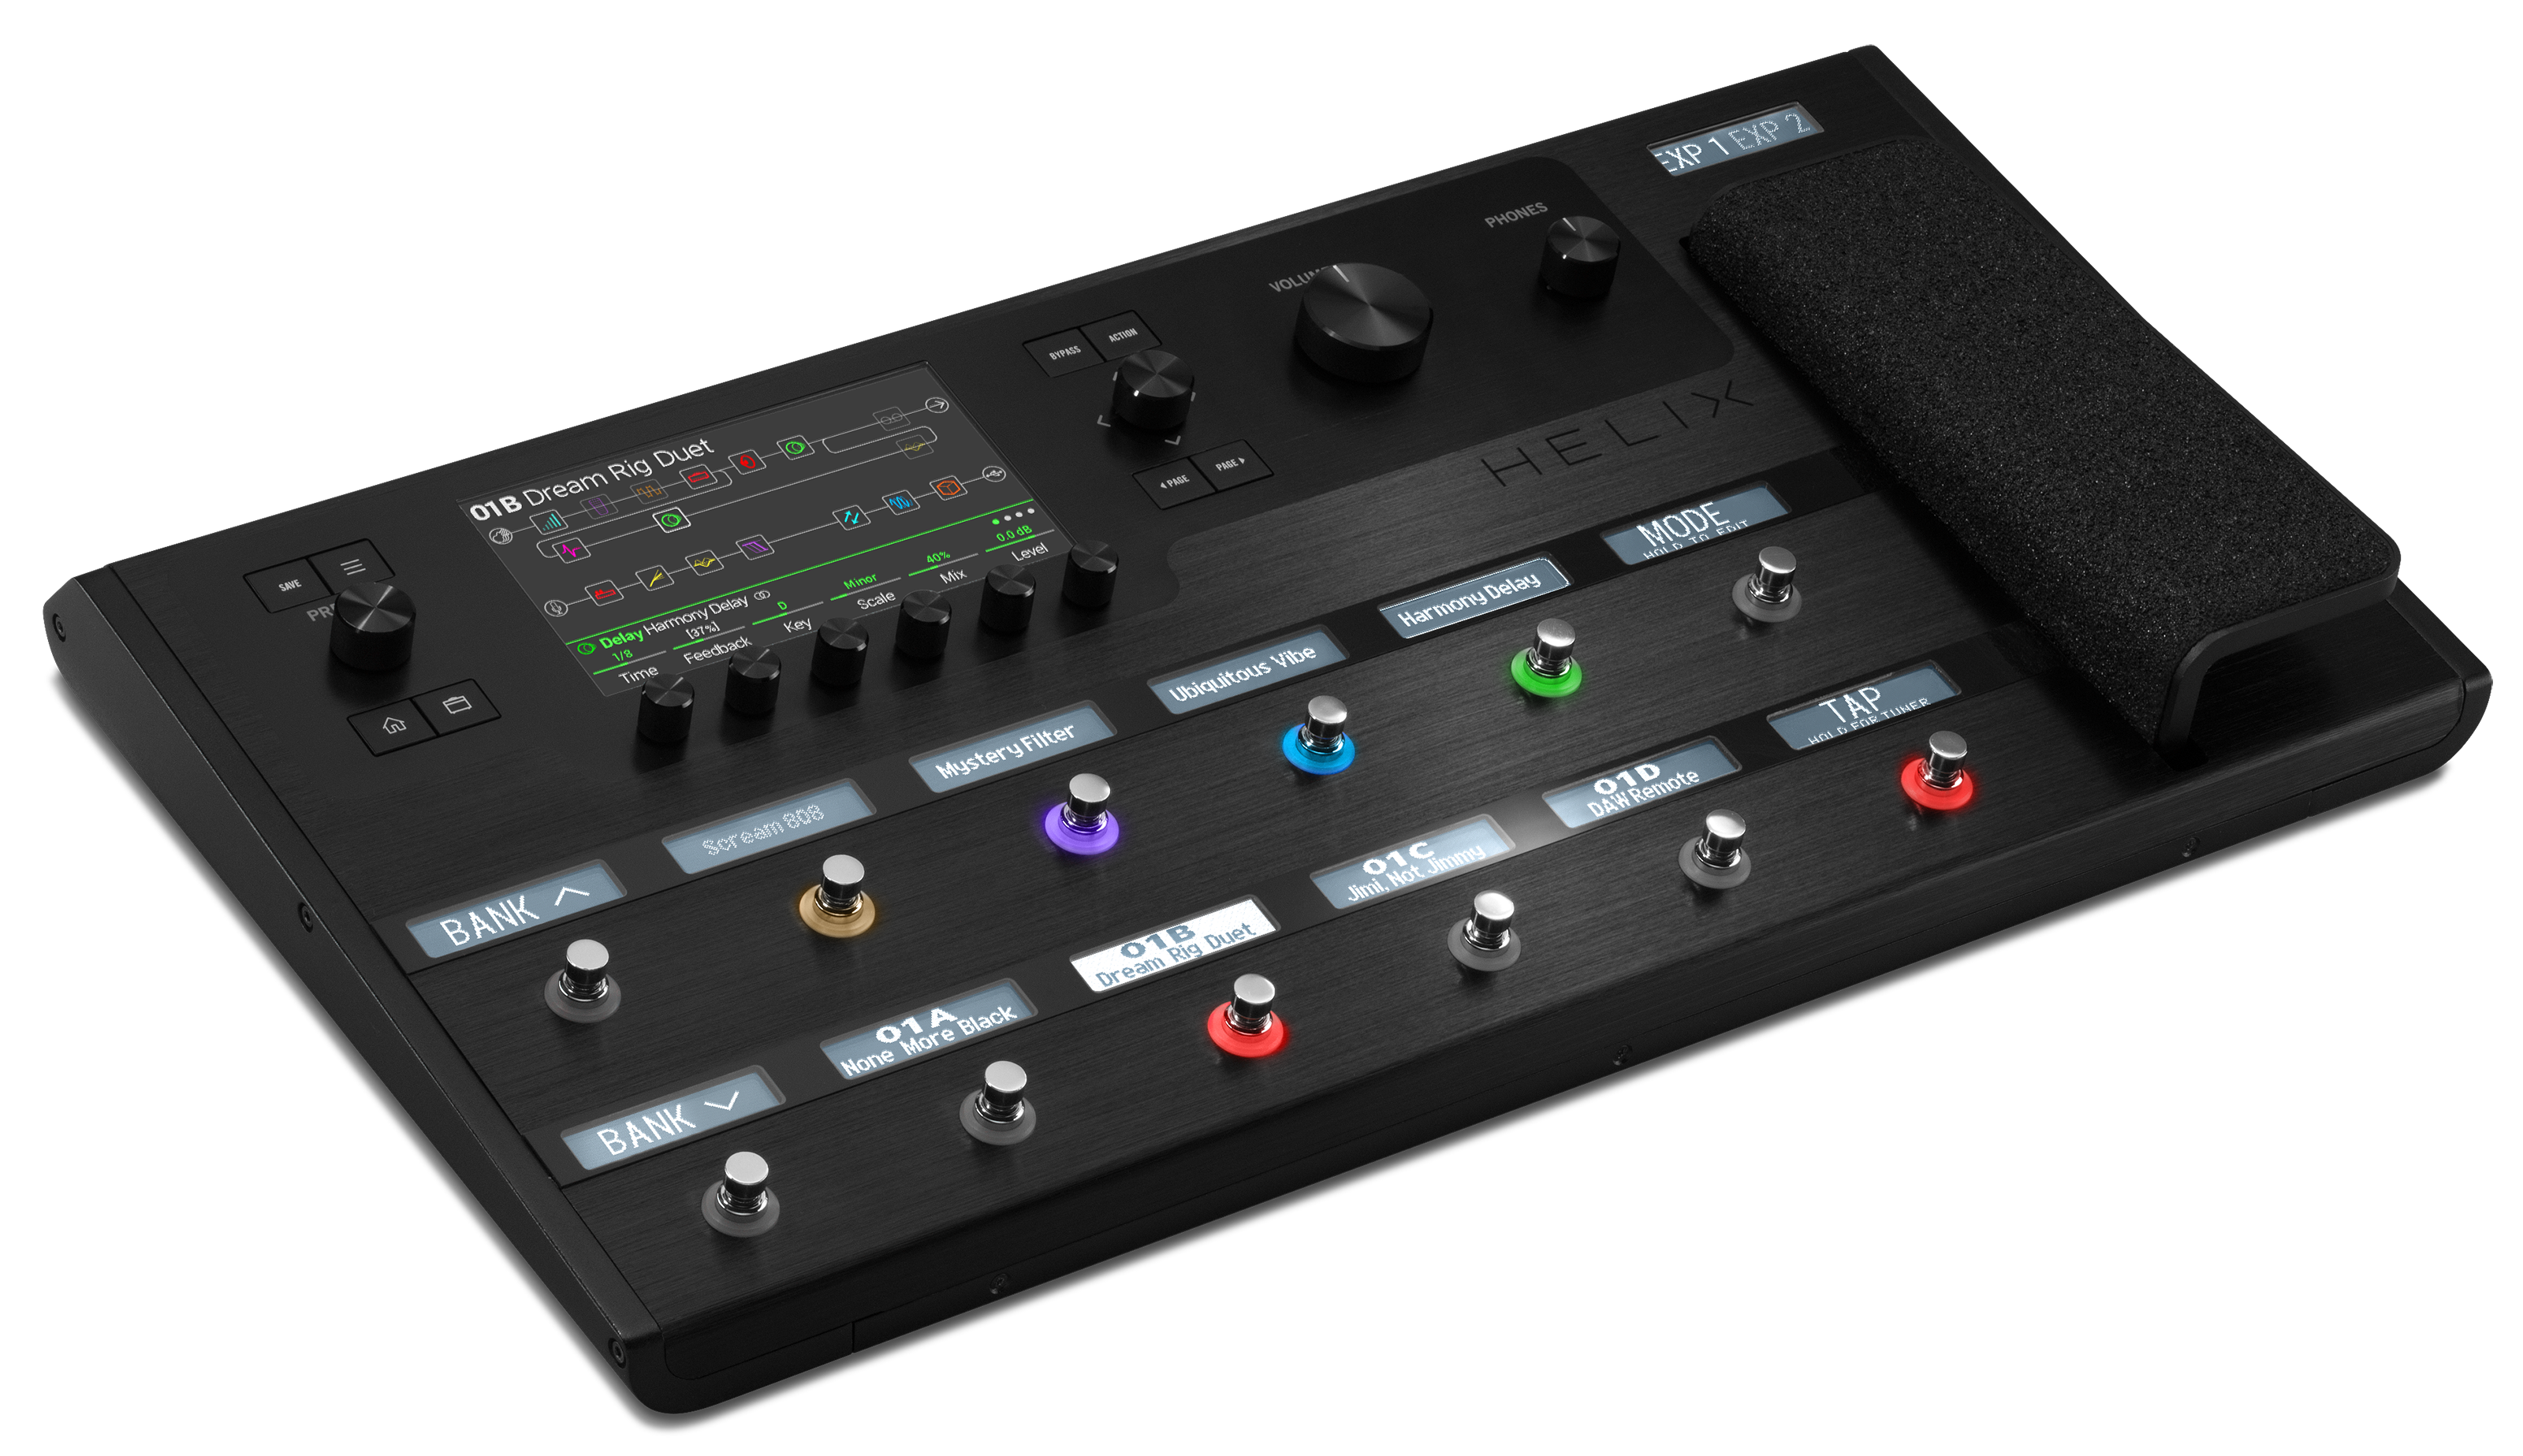
\includegraphics[width=0.5\textwidth]{img/helix.png}
\end{center}

\par{The application of DSP in guitar effects pedals is nothing new, and is growing in popularity as advancements in the industry are growing, with effects becoming more accurate to their analog counterparts. Products like the Quad Cortex\cite{quadcortex} and the Line 6 Helix\cite{line6helix} are currently being offered to players, and these all-in-one solutions have expansive libraries of effects, as well as built-in loopers. These products can also be updated with new presets that emulate pre-existing analog gear. This type of flexibility is advantageous, and offers the ability for players to achieve tones without spending exorbitant amounts of money on the vintage analog gear. This amount of flexibility would be ideal to include in the AxeTron, and would allow for further expansion of the unit, as opposed to making an entirely analog effects module that would be difficult to change down the road. }

\printbibliography

\end{document}

%%%%%%%%%%%%%%%%%%%%%%%%%%%%%%%%%%%%%%%%

% Copyright Remarks:
%--------------------

% Copyright holder: Vebjørn S. Førde, copyright: CC BY 4.0
% Note: The author of this template is also the copyright holder.

% Below is an explanation of the CC BY 4.0. Additional statements/ 
% clarifications made by the author/copyright holder are marked with *.

% YOU ARE FREE TO:
% Share — copy and redistribute the material in any medium or format
% Adapt — remix, transform, and build upon the material
% for any purpose, even commercially.

% UNDER THE FOLLOWING TERMS:
% Attribution* — You must give appropriate credit, provide a link to the license,
% and indicate if changes were made. You may do so in any reasonable manner, but 
% not in any way that suggests the licensor endorses you or your use.

% *Note: 
% Attribution NOT NEEDED for: 
%       - PDF distibution (like sharing your PDF document)
%       - Use of (dummy)text and images provided in the template (obviously)
%       - Distributing parts of the template, and not the template as a whole
% I am not really concerned with being given credit. As long as you do not 
% claim to have made the template yourself in distributing it further, I have
% no complaints.

% No additional restrictions — You may not apply legal terms or technological 
% measures that legally restrict others from doing anything the license permits.

% NOTICES:
% No warranties are given.

% Disclaimer* (added by copyright holder):
% THE SOFTWARE IS PROVIDED "AS IS", WITHOUT WARRANTY OF ANY KIND, EXPRESS OR
% IMPLIED, INCLUDING BUT NOT LIMITED TO THE WARRANTIES OF MERCHANTABILITY,
% FITNESS FOR A PARTICULAR PURPOSE AND NONINFRINGEMENT. IN NO EVENT SHALL THE
% AUTHORS OR COPYRIGHT HOLDERS BE LIABLE FOR ANY CLAIM, DAMAGES OR OTHER
% LIABILITY, WHETHER IN AN ACTION OF CONTRACT, TORT OR OTHERWISE, ARISING FROM,
% OUT OF OR IN CONNECTION WITH THE SOFTWARE OR THE USE OR OTHER DEALINGS IN THE
% SOFTWARE.

% Read more about CC BY 4.0:
% https://creativecommons.org/licenses/by/4.0/